\documentclass{article}

% Symbols
%\usepackage{recycle}
\usepackage{amsfonts, amsthm}
\usepackage{upgreek}
\usepackage{physics}
\usepackage{cancel}
\usepackage{amssymb, latexsym, amsmath}

%Algorithms
\usepackage[ruled,lined,linesnumbered,commentsnumbered]{algorithm2e}

%% Identación
\setlength{\parindent}{0cm}

% Código
\newcommand{\code}[1]{\textcolor{white!25!black}{\texttt{#1}}}
\usepackage{listings}

%AMS
\usepackage{amsthm}
\newtheorem{algo-thm}{Algoritmo}

% Proof
\renewcommand*{\proofname}{\textbf{Demostraci\'on:}}

% Graphics
\usepackage{graphicx}
\usepackage{pgf}

% Color a letras.
%\usepackage[usenames,dvipsnames,svgnames,table]{xcolor}

% Tikz
\usepackage{tkz-graph}
\usepackage{tikz}
\usetikzlibrary{arrows,automata}
\usepackage{tikz}
\usetikzlibrary{arrows,automata}
%\usetikzlibrary[topaths]

% Def. Dr. César.
\usetikzlibrary{shapes,calc}
\tikzstyle{edge}=[shorten <=2pt, shorten >=2pt, >=stealth, line width=1.1pt]
\tikzstyle{blueE}=[shorten <=2pt, shorten >=2pt, >=stealth, line width=1.5pt, blue]
\tikzstyle{blackV}=[circle, fill=black, minimum size=6pt, inner sep=0pt, outer sep=0pt]
\tikzstyle{blueV}=[circle, fill=blue, draw, minimum size=6pt, line width=0.75pt, inner sep=0pt, outer sep=0pt]
\tikzstyle{redV}=[circle, fill=red, draw, minimum size=6pt, line width=0.75pt, inner sep=0pt, outer sep=0pt]
\tikzstyle{redSV}=[semicircle, fill=red, minimum size=3pt, inner sep=0pt, outer sep=0pt, rotate=225]
\tikzstyle{blueSV}=[semicircle, fill=blue, minimum size=3pt, inner sep=0pt, outer sep=0pt, rotate=225]
\tikzstyle{blackSV}=[semicircle, fill=black, minimum size=3pt, inner sep=0pt, outer sep=0pt, rotate=225]
\tikzstyle{vertex}=[circle, draw, minimum size=6pt, line width=0.75pt, inner sep=0pt, outer sep=0pt]

% Margins
\addtolength{\voffset}{-1.5cm}
\addtolength{\hoffset}{-1.5cm}
\addtolength{\textwidth}{3cm}
\addtolength{\textheight}{3cm}

%\usepackage{geometry}
%\addtolength{\hoffset}{0cm}
%\addtolength{\textwidth}{0cm}
%\addtolength{\voffset}{0cm}
%\addtolength{\textheight}{1cm}

%Header-Footer
\usepackage{fancyhdr}
\renewcommand{\headrulewidth}{1pt}

\newcommand{\set}[1]{
  \left\{ #1 \right\}
}

%\pagenumbering{gobble} -- Este comando
%                       -- quita el número de página.
\footskip = 50pt
\renewcommand{\headrulewidth}{1pt}

\pagestyle{fancyplain}

\begin{document}
\title{UNIVERSIDAD AUT\'ONOMA DE M\'EXICO\\ Facultad de Ciencias}
\author{Autores:
  \\ Fernanda Villaf\'an Flores
  \\ Fernando Alvarado Palacios
  \\ Adri\'an Aguilera Moreno}
\date{}
\maketitle
\begin{center}
  
\includegraphics[scale=0.20]{../Imagen/Portada.jpg}\\[0.4cm]
  \Large
  \bf{Gr\'aficas y Juegos}
  \normalsize
\end{center}
\newpage
\fancyhead[r]{ Gr\'aficas y Juegos 2022-1}
%%%%%%%%%%%%%%%%%%%%%%%%%%%%%%%%%%%%%%%%%%%%%%%%%%%%%
\section*{\LARGE{Tarea 7}}
\begin{enumerate}
\item \begin{enumerate}
  %%%%%%%%%%%%%%%%%%%%%%%%%%%%%%%%% Ejercicio 01 %%%%%%%%%%%%%%%%%%%%%%%%%%%%%%%%%
  %~~~~~~~~~~~~~~~~~~~~~~~~~~~~~~~~ inciso (a)
\item Demuestre que si $G$ tiene di\'ametro mayor que $3$ (posiblemente
  infinito), entonces $\overline{G}$ tiene di\'ametro menor que $3$.
  Concluya que si $G$ es inconexa, entonces $\overline{G}$ es conexa.
   %~~~~~~~~~~~~~~~~~~~~~~~~~~~~~~~~ inciso (b)
\item Una gr\'afica $G$ es autocomplementaria si $G \cong \overline{G}$.
  Demuestre que si $G$ es autocomplementaria, entonces $|V|
  \stackrel{4}{\equiv} 0$ o $|V| \stackrel{4}{\equiv} 1$.
\end{enumerate}
  %%%%%%%%%%%%%%%%%%%%%%%%%%%%%%%%% Ejercicio 02 %%%%%%%%%%%%%%%%%%%%%%%%%%%%%%%%%
\item Un {\em orden topol\'ogico} de una digr\'afica $D$ es un orden lineal de
  sus v\'ertices tal que para cada flecha $a$ de $D$, la cola de $a$ precede a
  su cabeza en el orden.
  \begin{enumerate}
    %~~~~~~~~~~~~~~~~~~~~~~~~~~~~~~~~ inciso (a)
  \item Demuestre que toda digr\'afica ac\'iclica tiene al menos una fuente
    (v\'ertice de ingrado $0$) y un sumidero (v\'ertice de exgrado $0$).
    \begin{proof}
      Procedamos por reducci\'on al absurdo. Sea $D$ una digr\'afica ac\'iclica
      con $\delta^+ > 0$ y $\delta^- > 0$, esto es que, para cada $v \in V_D$ hay
      una flecha que le ``\textit{pega}''\footnote{Una arista incide en $v$ y $v$
        es la cabeza.} a $v$ y otra que ``\textit{sale}''\footnote{Una arista que
        inicia en $v$ con direcci\'on a otro v\'ertice.} de $v$. Tomemos la
      trayectoria $\vec{T}$ m\'as larga en $D$ y sea $x \in V_D$ el \'ultimo
      v\'ertice de $\vec{T}$, luego en $x$ \textit{sale} una arista hacia alg\'un
      otro v\'ertice en $\vec{T}$ [pues si saliera hacia alg\'un otro v\'ertice que
        no este en $\vec{T}$, llegariamos a que $\vec{T}$ no es de longitud m\'axima!!],
      as\'i $\vec{T}xy$ claramente contiene un ciclo, esto implica que $D$ contiene
      un ciclo!!, he aqu\'i una contradicci\'on de suponer que $D$ no contiene ciclos.
      
      \hspace*{2cm} $\therefore\;$ Si $D$ es ac\'iclica tiene al menos una fuente y un sumidero.
    \end{proof}
    %~~~~~~~~~~~~~~~~~~~~~~~~~~~~~~~~ inciso (b)
  \item Deduzca que una digr\'afica admite un orden topol\'ogico si y s\'olo
    si es ac\'iclica.
    \begin{proof}
      Para este inciso analicemos $2$ posibles casos:
      \begin{itemize}
      \item[$\Rightarrow$)] Procedamos por reducci\'on al absurdo. Sea $D$ una
        digr\'afica tal que admite un orden topol\'ogico. Supongamos que $D$
        contiene al menos un ciclo $C$, entonces existe un $x \in V_D$ tal que
        $\{x\} \subset C$ y $x$ es un v\'ertice inicial y final en $C$, luego
        existe $y \in V_D : \{y\} \subset C$ tal que $\vec{yx}$ es una arista,
        por tanto $y < x$ [esto es que $y$ precede a $x$ en el orden]. N\'otese
        que hay una trayectoria $\vec{T}$ que va de $x$ a $y$ en $C$, as\'i
        $x < y$!! [esto es que $x$ precede a $y$ en el orden], he aqu\'i una
        contradicci\'on de suponer que $D$ admite un orden topol\'ogico.
        \[
        \therefore \text{ Si $D$ admite un orden topol\'ogico}
        \Rightarrow D \text{ es ac\'iclica.}
        \]
      \item[$\Leftarrow$)] Por el inciso $(a)$ sabemos que $D$ tiene al menos
        una \textit{fuente} y un \textit{sumidero}, tomemos una componente
        conexa en $D$ y veamos que si los v\'ertices $x$ es \textit{fuente}
        e $y$ es \textit{sumidero}, entonces la trayectoria de $x$ a $y$ es
        un orden topol\'ogico, si hay m\'as de una \textit{fuente} o m\'as de
        un \textit{sumidero}, cada trayectoria entre una \textit{fuente} y un
        \textit{sumidero} es un orden topol\'ogico [pues de no serlo, dos flechas
          distintas provenientes de una misma fuente incidir\'ian en alg\'un
          v\'ertice en com\'un, lo que implicar\'ia que $D$ contiene un ciclo!!],
        as\'i la componente conexa admite un orden topol\'ogico y esto pasa
        para cualquier componente conexa en $D$.
        \[
        \therefore \text{ Si $D$ es ac\'iclica}
        \Rightarrow D \text{ admite un orden topol\'ogico.}
        \]
      \end{itemize}
      \hspace*{1.3cm} $\therefore\;$ Una digr\'afica admite un orden
      topol\'ogico si y s\'olo si es ac\'iclica.
    \end{proof}
    %~~~~~~~~~~~~~~~~~~~~~~~~~~~~~~~~ inciso (c)
  \item Exhiba un algoritmo de tiempo a lo m\'as cuadr\'atico para encontrar
    un orden topol\'ogico en una digr\'afica ac\'iclica.
  \end{enumerate}
\end{enumerate}
%%********************************** Algoritmo 1: Orden Topol\'ogico.
A continuaci\'on se muestra el algoritmo\footnote{Tome en cuenta que suponemos
  que $D$ se pasa como par\'ametro con valores nulos en sus v\'ertices.} requerido:

\begin{algorithm}[H]
  \SetAlgorithmName{}{}%Orden Topol\'ogico}{}
  \DontPrintSemicolon
  \SetKwData{False}{false}\SetKwData{True}{true}
  \SetKwFunction{New}{new}\SetKwFunction{End}{end}\SetKwFunction{Used}{used}
  \SetKwInOut{Input}{input}\SetKwInOut{Output}{output}
  
  \KwIn{Una digr\'afica $D$ ac\'iclica.}
  \KwOut{Un orden topol\'ogico admitido en $D$ basado en n\'umeros.}
  \BlankLine {
    \For{$v \in V_D$ \textnormal{\textbf{and}} $d^-(v) = 0$}{
      $v \gets$ 0\;
    }
    \For{$v \in V_D$}{
      \If{$v \not= 0$}{
        \code{temp} $\gets 0$\;
        \For{$u\in V_D: u$\textnormal{ es antecesor de} $v$ \textnormal{en} $D$
          \textnormal{\textbf{and}} $u \not=$ \textnormal{\code{null}}}{
          \If{\textnormal{\code{temp}} $< u$}{
            \code{temp} $\gets u$
          }
        }
        $v \gets temp + 1$\;
        \For{$u\in V_D: u$\textnormal{ es sucesor de} $v$ \textnormal{en} $D$
          \textnormal{\textbf{and}} $u \not=$ \textnormal{\code{null}}}{
          \If{$u < v$}{
            $u \gets v + 1$ 
          }
        }
      }
    }
  }
  {\Return $D$}
  \caption{TopologicalOrder$(D;D)$} \label{TopologicalOrder}%\textnormal{new}
  \DecMargin{1em}
\end{algorithm}
%\newpage
\begin{enumerate}
  %%%%%%%%%%%%%%%%%%%%%%%%%%%%%%%%% Ejercicio 03 %%%%%%%%%%%%%%%%%%%%%%%%%%%%%%%%%
\item[3.] Demuestre que cada uno de los siguientes problemas est\'a en la clase
  $NP$ exhibiendo un certificado y un algoritmo de tiempo polinomial para
  verificar el certificado (escriba el algoritmo utilizando pseudo c\'odigo
  como el visto en clase; s\'olo est\'a permitido el uso de las estructuras de
  control {\bf if}, {\bf while} y {\bf for}).   Demuestre que su algoritmo
  usa tiempo polinomial.
  \begin{enumerate}
    %~~~~~~~~~~~~~~~~~~~~~~~~~~~~~~~~ inciso (a)
  \item \textsc{Hamilton Cycle}.
    %~~~~~~~~~~~~~~~~~~~~~~~~~~~~~~~~ inciso (b)
  \item \textsc{Vertex Cover}.
    %~~~~~~~~~~~~~~~~~~~~~~~~~~~~~~~~ inciso (c)
  \item \textsc{Colouring}.
    %~~~~~~~~~~~~~~~~~~~~~~~~~~~~~~~~ inciso (d)
  \item \textsc{Dominating Set}.
  \end{enumerate}
\end{enumerate}
\textbf{Soluci\'on de (a):}
A continuaci\'on se da un certificado para una gr\'afica que contiene un ciclo hamiltoniano:

%%%%%%%%%%%%%%%%%%%%%%%%%%%%%%%%%%%%%%%%%%%%%%%%%%%%%%%%%%%%%%%%%%%%%%%%%% Sí-certificado:
\begin{center}
  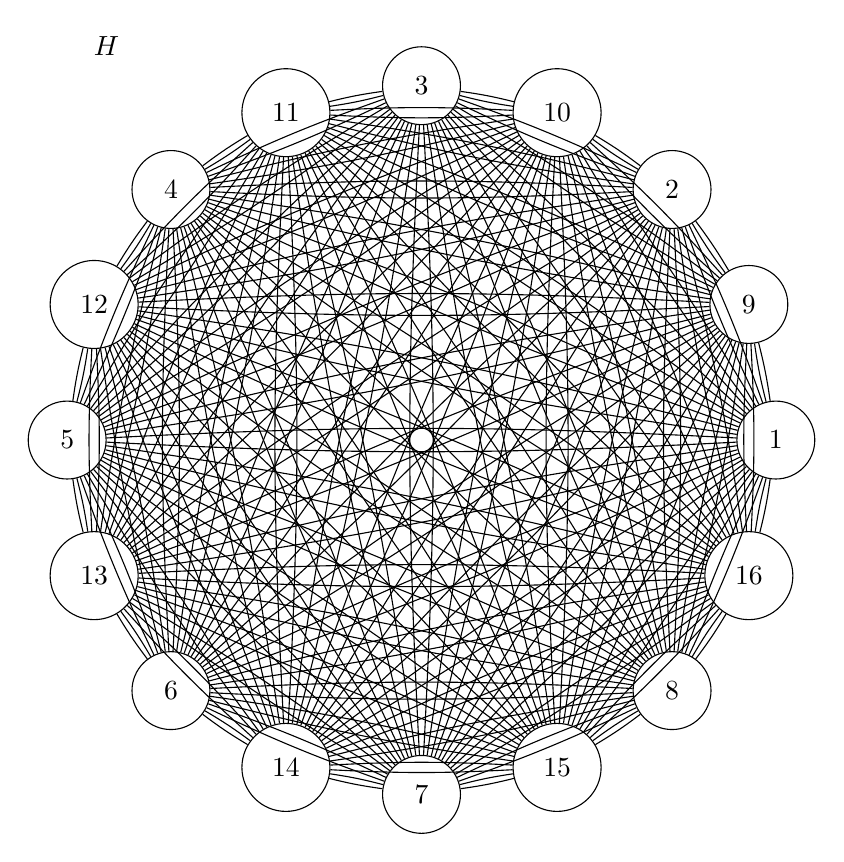
\begin{tikzpicture}[transform shape]
    \foreach \x in {1,...,16}{%
      \pgfmathparse{(\x-1)*45+floor(\x/9)*22.5}
      \node[draw,circle,inner sep=0.25cm] (N-\x) at (\pgfmathresult:4.5cm) {$\x$};%5.4cm
    } 
    \foreach \x [count=\xi from 1] in {2,...,16}{%
      \foreach \y in {\x,...,16}{%
        \path (N-\xi) edge[-,bend right=3] (N-\y)  edge[-,bend left=3] (N-\y);
      }
    }
    \node (L) at (-4,5){$H$};   
  \end{tikzpicture}
\end{center}

y $S = (v_0, v_1, \dotsm, v_n, v_0) = (3, 10, 2, 9, 1, 16, 8, 15, 7, 14, 6, 13, 5, 12, 4, 11, 3)$
una \code{colecci\'on} que contiene los v\'ertices en sucesi\'on tal que est\'a sucesi\'on forma
un ciclo hamiltoniano en $H$.
%%%%%%%%%%%%%%%%%%%%%%%%%%%%%%%%%%%%%%%%%%%%%%%%%%%%%%%%%%%%%%%%%%%%%%%%%%
As\'i, nuestro algoritmo es el siguiente:

\begin{algorithm}[H]
  \SetAlgorithmName{}{}
  \DontPrintSemicolon
  \SetKwData{False}{false}\SetKwData{True}{true}
  \SetKwFunction{New}{new}\SetKwFunction{End}{end}\SetKwFunction{Used}{used}
  \SetKwInOut{Input}{input}\SetKwInOut{Output}{output}
  \KwIn{Una gr\'afica $H$ y una colecci\'on $S$ que contiene a la sucesi\'on de v\'ertices que
    representar\'a el ciclo hamiltoniano en $H$.}
  \KwOut{\code{TRUE} o \code{FALSE} dependiendo si $S$ es un ciclo hamiltoniano en $H$.}
  \BlankLine {
    \For{$v \in S$}{
      \code{siguiente}$= 0$\;
      \While{\textnormal{\code{siguiente}} $< |V_H|$}{
        $u \gets $ S(\code{siguiente})\;
        \code{siguiente} $\gets$ \code{siguiente} + 1\;
        \If{$vu \notin E_H$}{
          {\Return \code{false}\;}
        }
      }
    }
    \If{$S(0) \not= $S($|V_H - 1|$)}{
      {\Return \code{false}\;}
    }
    \For{$v \in S$}{
      \If{$v \notin V_H$}{
        {\Return false\;}
      }
    }
  } {\Return \code{true}\;}
  \caption{HamiltonCycle$(\big<H,S\big>;\code{true}/\code{false})$} \label{HamiltonCycle}
  \DecMargin{1em}
\end{algorithm}

\textbf{Soluci\'on de (b):}
A continuaci\'on se da un certificado para una gr\'afica que contiene un covertura de v\'ertices:
%%%%%%%%%%%%%%%%%%%%%%%%%%%%%%%%%%%%%%%%%%%%%%%%%%%%%%%%%%%%%%%%%%%%%%%%%% Sí-certificado:
\begin{figure}[ht!]
  \centering
  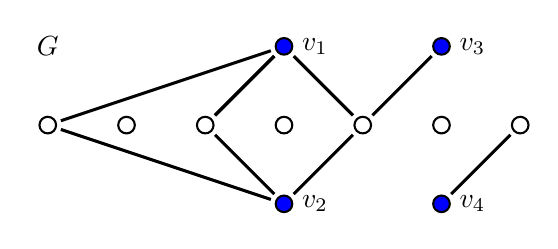
\begin{tikzpicture}
    \foreach \i in {-1,0,1,...,5}
    \node(\i) [vertex] at (\i*1, -2){};
    \node(6) [blueV, label=0:$v_1$] at (2, -1){};
    \node(7) [blueV, label=0:$v_2$] at (2, -3){};
    \node(8) [blueV, label=0:$v_3$] at (4, -1){};
    \node(9) [blueV, label=0:$v_4$] at (4, -3){};
    \draw[edge] (1) to (6);
    \draw[edge] (1) to (7);
    \draw[edge] (3) to (6);
    \draw[edge] (3) to (7);
    \draw[edge] (1) to (6);
    \draw[edge] (-1) to (6);
    \draw[edge] (-1) to (7);
    \draw[edge] (5) to (9);
    \draw[edge] (3) to (8);
    \node (L) at (-1,-1){$G$};   
  \end{tikzpicture}
\end{figure}
%%%%%%%%%%%%%%%%%%%%%%%%%%%%%%%%%%%%%%%%%%%%%%%%%%%%%%%%%%%%%%%%%%%%%%%%%%

con $S = (v_1,v_2v_3,v_4)$ una cubierta de v\'ertices en $G$. As\'i
nuestro algoritmo ser\'ia el que a continuaci\'on se muestra:

\begin{algorithm}[H]
  \SetAlgorithmName{}{}
  \DontPrintSemicolon
  \SetKwData{False}{false}\SetKwData{True}{true}
  \SetKwFunction{New}{new}\SetKwFunction{End}{end}\SetKwFunction{Used}{used}
  \SetKwInOut{Input}{input}\SetKwInOut{Output}{output}
  \KwIn{Una gr\'afica $G$ y una \code{colecci\'on} $S$ que contiene a la sucesi\'on
  que conforma la covertura de v\'ertices en $G$.}
  \KwOut{\code{TRUE} o \code{FALSE} dependiendo si $S$ es una covertura de v\'ertices en $G$.}
  \BlankLine {
    \code{contador} $\gets 0$\;
    \For{$v \in S$}{
      \If{$v \notin V_G$}{
        {\Return \code{false}\;}
      }
      \For{$u \in V_G$}{
        \If{$vu \in E_G$}{
          \code{contador} $\gets$ \code{contador} + 1\;
        }
      }
    }
    \If{\textnormal{\code{contador}}$\not= |V_G|$}{
      {\Return \code{false}\;}
    }
  } {\Return \code{true}\;}
  \caption{VertexCover$(\big<G,S\big>;\code{true}/\code{false})$} \label{VertexCover}
  \DecMargin{1em}
\end{algorithm}

\textbf{Soluci\'on de (c):}
A continuaci\'on se muestra un certificado para una gr\'afica que admite una coloraci\'on:
%%%%%%%%%%%%%%%%%%%%%%%%%%%%%%%%%%%%%%%%%%%%%%%%%%%%%%%%%%%%%%%%%%%%%%%%%% Sí-certificado:
\begin{figure}[ht!]
  \centering
  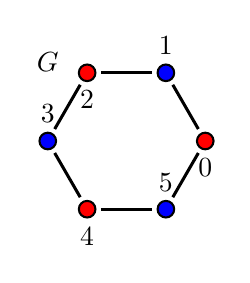
\begin{tikzpicture}
    \foreach \i in {0,2,4}
    \node (\i) [redV, label=270:$\i$]  at ({(360/6)*\i}:1){};
    \foreach \i in {1,3,5}
    \node (\i) [blueV, label=90:$\i$] at ({(360/6)*\i}:1){};
    
    \foreach \i in {0,...,5}
    \draw [edge] let \n1={int(mod(\i+1,6))} in (\i) to (\n1);
    
    \node (L) at (-1,1){$G$};
  \end{tikzpicture}
\end{figure}
%%%%%%%%%%%%%%%%%%%%%%%%%%%%%%%%%%%%%%%%%%%%%%%%%%%%%%%%%%%%%%%%%%%%%%%%%% 

con $S = (1R,3R,5R,0A,2A,4A)$ una coloraci\'on de v\'ertices en $G$. Luego,
nuestro algoritmo ser\'ia el que a continuaci\'on se muestra:

\begin{algorithm}[H]
  \SetAlgorithmName{}{}
  \DontPrintSemicolon
  \SetKwData{False}{false}\SetKwData{True}{true}
  \SetKwFunction{New}{new}\SetKwFunction{End}{end}\SetKwFunction{Used}{used}
  \SetKwInOut{Input}{input}\SetKwInOut{Output}{output}
  \KwIn{Una gr\'afica $G$ y una \code{colecci\'on} $S$ que contiene a la sucesi\'on
    que conforma la coloraci\'on de v\'ertices en $G$.}
  \KwOut{\code{TRUE} o \code{FALSE} dependiendo si $S$ es una coloraci\'on de v\'ertices en $G$.}
  \BlankLine {
    \If{$|S| = |V_G|$}{
      {\Return false\;}
    }
    \For{$v \in S$}{
      \If{$v \notin V_G$}{
        {\Return \code{false}\;}
      }
      \For{$u \in S$}{
        \If{$v$ \textnormal{tiene el mismo color que} $u$}{
          \If{$uv \in E_G$}{
            {\Return \code{false}\;}
          }
        }
      }
    }
  } {\Return \code{true}\;}
  \caption{Colouring$(\big<G,S\big>;\code{true}/\code{false})$} \label{Colouring}
  \DecMargin{1em}
\end{algorithm}

\textbf{Soluci\'on de (d):}
A continuaci\'on se muestra un certificado para una gr\'afica que admite una coloraci\'on:
%%%%%%%%%%%%%%%%%%%%%%%%%%%%%%%%%%%%%%%%%%%%%%%%%%%%%%%%%%%%%%%%%%%%%%%%%% Sí-certificado:
\begin{figure}[ht!]
  \centering
  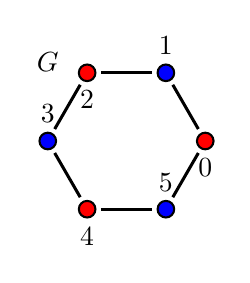
\begin{tikzpicture}
    \foreach \i in {0,2,4}
    \node (\i) [redV, label=270:$\i$]  at ({(360/6)*\i}:1){};
    \foreach \i in {1,3,5}
    \node (\i) [blueV, label=90:$\i$] at ({(360/6)*\i}:1){};
    
    \foreach \i in {0,...,5}
    \draw [edge] let \n1={int(mod(\i+1,6))} in (\i) to (\n1);
    
    \node (L) at (-1,1){$G$};
  \end{tikzpicture}
\end{figure}
%%%%%%%%%%%%%%%%%%%%%%%%%%%%%%%%%%%%%%%%%%%%%%%%%%%%%%%%%%%%%%%%%%%%%%%%%% 

con $S = (1R,3R,5R,0A,2A,4A)$ una coloraci\'on de v\'ertices en $G$. Luego,
nuestro algoritmo ser\'ia el que a continuaci\'on se muestra:


%%%%%%%%%%%%%%%%%%%%%%%%%%%%%%%%%%%%%%%% Extras %%%%%%%%%%%%%%%%%%%%%%%%%%%%%%%%%%%%%%%%%%
\subsection*{Puntos extra}
\begin{enumerate}
\item Demuestre que toda digr\'afica sin lazos admite una
  descomposici\'on en dos digr\'aficas ac\'iclicas, es decir, que
  existen $D_1$ y $D_2$ subdigr\'aficas de $D$, ac\'iclicas y
  tales que $D_1 \cup D_2 = D$ y $A_{D_1} \cap A_{D_2} =
  \varnothing$.

\item Un torneo es una digr\'afica en la que entre cualesquiera
  dos v\'ertices existe una \'unica flecha.   Demuestre que todo
  torneo es fuertemente conexo o puede transformarse en un
  torneo fuertemente conexo al reorientar exactamente una
  flecha.

\item Demuestre que una digr\'afica es fuertemente conexa si
  y s\'olo si contiene un camino cerrado generador.

\item Demuestre que si $l, m$ y $n$ son enteros con $0 < l \le
  m \le n$, entonces existe una gr\'afica simple $G$ con $\kappa
  = l$, $\kappa' = m$ y $\delta = n$.

  \begin{proof} 
    Sean l, m, n perteneciente a los Enteros  y G una gráfica con K=l, k'=m y $\delta$=n, tenemos que $0<k$ ya que una gráfica no puede tener conexidad menor que 0  $\rightarrow$ por proposición demostrada en clase esta gráfica tendra la desigualdad $0<k \leqslant k' \leqslant \delta $ sustituyendo los valores  $0 < l \leqslant m \leqslant n$
    
    Por lo tanto existe la grafica (ya que la proposicion demostrada en clase era un para todo y el paratodo implica el existe)
    
    \end{proof}

\end{enumerate}
\end{document}
